% 译自 arXiv:2306.13589v2 原 tex 第 4190–4389 行
\subsection{一维的同调镜像对称}\label{ch7.3}


我们终于来到椭圆曲线的同调镜像对称的陈述，其恰当的表述见 \cite[定理 4.1]{[Kre00]}。值得指出的是，由两条椭圆曲线构成的镜像对与经典镜像对称的预测相符：对其 Hodge 菱形的分析表明椭圆曲线是自对偶的（见 \cite[例 7.10]{[Imp21]}）。  

\begin{Thm}\label{HMSindim1}
设 $\tau\in\mathbb{C}$ 满足 $\mathfrak{Im}(\tau)>0$。则存在等价
\begin{equation}
	\mathsf{E}_\tau:\mathsf{D^b}(E_\tau)\rightarrow\mathscr{F\!K}^0(E^\tau)
\end{equation}
它与相应的平移函子相容。
\end{Thm}

\begin{proof}(\textit{略述})
我们首先在对象上定义 $\mathsf{E}_\tau$。由注 \ref{indecomposabletorsion}，只需关注不可分解凝聚层 $\mathcal{E}\in\textup{obj}(\mathsf{Coh}(E_\tau;{}_{\mathcal{O}_{E_\tau}}\!\mathsf{Mod}))$；由推论 \ref{indecompocoherentonell}，它们要么是不可分解向量丛，要么是支撑于一点的不可分解挠层。我们按顺序进行。
\begin{itemize}[leftmargin=0.5cm]
	\item 首先设 $\mathcal{E}$ 是形如 $\mathcal{E}=\mathcal{L}_\tau(\varphi)\otimes F_\tau(V,e^N)\in\text{obj}(\mathsf{D^b}(E_\tau))$ 的不可分解向量丛，其中 $\varphi=t_x^*\varphi_0\cdot\varphi_0^{n-1}$ 依命题 \ref{linebundleonell} 取定，$x=a\tau+b\in E_\tau$、$n\in\mathbb{Z}$，而不可分解的 $F_\tau(V,e^N)$ 依定义 \ref{unipotentvectorbundle} 取定。则我们置 
	\[
	\mathsf{E}_\tau(\mathcal{L}_\tau(\varphi)\otimes F_\tau(V,e^N))\coloneqq(\Lambda,\alpha,M)\in\text{obj}(\mathscr{F\!K}^0(E^\tau))\,,
	\]
	其中 $\Lambda\coloneqq(a+t,(n-1)a+nt)/\mathbb{Z}^2$，$\alpha\in(-\frac{1}{2},\frac{1}{2}]$ 是使 $e^{i\pi\alpha}=\frac{1+in}{\sqrt{1+n^2}}$ 的唯一实数，且 $M\coloneqq e^{-2\pi i b\,\text{id}_V + N}$。
	
	\item 现设 $\pi_r:E_{r\tau}\rightarrow E_\tau$ 为同源，且 $\mathcal{E}=\pi_{r*}(\mathcal{L}_{r\tau}(\varphi)\otimes F_{r\tau}(V,e^N))\in\text{obj}(\mathsf{D^b}(E_{\tau}))$——由定理 \ref{AtiyahThm}，这是 $E_\tau$ 上任意不可分解向量丛所取的一般形式。于是，对定义 \ref{FukayaKontsevichcat} 中的 $p_r:E^{r\tau}\rightarrow E^\tau$，我们置
	\[
	\mathsf{E}_\tau(\mathcal{E})\coloneqq p_{r*}\mathsf{E}_{r\tau}(\mathcal{E})=(\Lambda,\alpha,M)\in\text{obj}(\mathscr{F\!K}^0(E^\tau))\,,
	\]
	其中 $\Lambda\coloneqq\big(a+t,(\frac{n}{r}-1)a+\frac{n}{r}t\big)/\mathbb{Z}^2$，$\alpha\in(-\frac{1}{2},\frac{1}{2}]$ 满足 $e^{i\pi\alpha}=\frac{1+in/r}{\sqrt{1+n^2/r^2}}$，而同样 $M\coloneqq e^{-2\pi i b\,\text{id}_V + N}$。
	
	\item 若 $\mathcal{E}=\mathcal{S}(x,V,N)\in\text{obj}(\mathsf{D^b}(E_{\tau}))$ 是支撑于 $x=a\tau+b\in E_\tau$ 的挠层，则我们简单地置
	\[
	\mathsf{E}_\tau(\mathcal{S}(a\tau+b,V,N))\coloneqq((-a,t)/\mathbb{Z}^2,1/2,e^{2\pi i b\,\text{id}_V+N})
	\]
	（从而 $\Lambda$ 是一条经线环路）。   
\end{itemize}
为了在态射上定义 $\mathsf{E}_\tau$，只需建立映射
\[
(\mathsf{E}_\tau)_{\mathcal{E}_1,\mathcal{E}_2}:\text{Hom}_{\mathsf{D^b}(E_\tau)}(\mathcal{E}_1,\mathcal{E}_2[n])\rightarrow\text{Hom}_{\mathscr{F\!K}^0(E^\tau)}(\mathsf{E}_\tau(\mathcal{E}_1),\mathsf{E}_\tau(\mathcal{E}_2)[n])
\]
（对 $n=0,1$，其中 $\mathcal{E}_1,\mathcal{E}_2\in\text{obj}(\mathsf{D^b}(E_\tau))$ 任意）。但由引理 \ref{ellSerreduality} 与「辛」Serre 对偶 \eqref{sympSerreduality}，情形 $n=0$ 实际上已经足够。我们再次分步进行。
\begin{itemize}[leftmargin=0.5cm]
	\item 我们首先处理形如 $\mathcal{E}_i=\mathcal{L}_\tau(\varphi_i)\otimes F_\tau(V_i,e^{N_i})\in\text{obj}(\mathsf{D^b}(E_\tau))$ 的不可分解向量丛，其中 $\varphi_i=t_{x_i}^*\varphi_0\cdot\varphi_0^{n_i-1}$、$x_i=a_i\tau+b_i\in E_\tau$（$i=0,1$），使得 $\mathsf{E}_\tau(\mathcal{E}_i)=(\Lambda_i,\alpha_i,M_i)$ 且 $\Lambda_0\neq\Lambda_1$。由 \cite[命题 2]{[PZ00]}，对任何这样的凝聚层都存在同构 $H^0(\mathcal{L}_\tau(\varphi))\otimes V\cong H^0(\mathcal{L}_\tau(\varphi)\otimes F_\tau(V,e^{N}))$；把它应用于 $\varphi=\varphi_1\varphi_0^{-1}$ 与 $V=\text{Hom}(V_0,V_1)$，我们得到 $\text{Hom}_{\mathsf{D^b}(E_\tau)}(\mathcal{E}_1,\mathcal{E}_2)\cong H^0(\mathcal{L}_\tau(\varphi_1\varphi_0^{-1}))\otimes\text{Hom}(V_0,V_1)$（不妨设 $n_0<n_1$）。 
	\newline 于是，由 $\mathsf{E}_\tau$ 的线性性，只需在形如 $\theta\otimes f\in H^0(\mathcal{L}_\tau(\varphi_1\varphi_0^{-1}))\otimes\text{Hom}(V_0,V_1)$ 的元素上指定它即可，因为 theta 函数构成 $H^0(\mathcal{L}_\tau(\varphi_1\varphi_0^{-1}))$ 的一组基；按命题 \ref{linebundleonell}，我们具体需要给出 $t_{x_{01}}^*\theta[k/(n_1\!-\!n_0),0]((n_1\!-\!n_0)\tau,(n_1\!-\!n_0)z)$ 的指定，其中 $x_{01}=(x_1\!-\!x_0)/(n_1\!-\!n_0)$ 且 $0\leq k<n_1\!-\!n_0$。这一指定是
	\begin{small}\[
		t_{x_{01}}^*\theta\Big[\frac{k}{n_1\!-\!n_0},0\Big]\big((n_1\!-\!n_0)\tau,(n_1\!-\!n_0)z\big)\mapsto e_k\!\coloneqq\!\Big(\frac{a_1\!-\!a_0\!+\!k}{n_1\!-\!n_0},\frac{n_0a_1\!-\!n_1a_0\!+\!n_0k}{n_1\!-\!n_0}\Big)\,,
		\]\end{small}
	\!\!于是这些 $e_k$ 恰是 $\Lambda_0$ 与 $\Lambda_1$ 的交点。拉格朗日子流形重合的情形 $\Lambda_0=\Lambda_1$ 在 \cite{[Kre00]} 中处理。
	
	\item 现在我们想把 $\mathsf{E}_\tau$ 在态射上的定义推广到任意向量丛 $\pi_{r_i*}(\mathcal{E}_i)=\pi_{r_i*}(\mathcal{L}_{r_i\tau}(\varphi_i)\otimes F_{r_i\tau}(V_i,e^{N_i}))\in\text{obj}(\mathsf{D^b}(E_{\tau}))$，其中 $r_0,r_1>0$ 可以相等。其实我们并不推广；感兴趣的读者可在 \cite[定理 4.1]{[Kre00]} 的证明中读到这一步。
	
	\item 若 $\mathcal{E}_0=\mathcal{L}_\tau(\varphi_0)\otimes F_\tau(V_0,e^{N_0})$ 是不可分解向量丛，而 $\mathcal{E}_1=\mathcal{S}(x_1,V_1,N_1)\in\text{obj}(\mathsf{D^b}(E_\tau))$ 是支撑于 $x_1=a_1\tau+b_1\in E_\tau$ 的不可分解挠层，则相应的拉格朗日子流形恰交于一点，由此得到典范同构 $\text{Hom}_{\mathsf{D^b}(E_\tau)}(\mathcal{E}_0,\mathcal{E}_1)\cong\text{Hom}(V_0,V_1)\cong V_0^*\otimes V_1$ 与 $\text{Hom}_{\mathscr{F\!K}^0(E^\tau)}\cong\text{Hom}(V_0,V_1)$。于是 
	\begin{small}
		\begin{align*}
			&(\mathsf{E}_\tau)_{\mathcal{E}_0,\mathcal{E}_1}:V_0^*\otimes V_1\rightarrow V_0^*\otimes V_1\,, \\
			&(f_0,v_1)\mapsto e^{-\pi i(\tau(na_1^2+2a_0a_1)+2(a_1b_0+a_0b_1+na_1b_1))}e^{-(a_0+na_1)f_0\otimes N_1(v_1)+a_1N_0^*(f_0)\otimes v_1}.
		\end{align*}
	\end{small}
	\!\!此外，在更一般的 $\pi_{r_0*}(\mathcal{E}_0)=\pi_{r_0*}(\mathcal{L}_{r_0\tau}(\varphi_0)\otimes F_{r_0\tau}(V_0,e^{N_0}))$ 上，为定义下图中虚线箭头 $(\mathsf{E}_\tau)_{\pi_{r_0*}(\mathcal{E}_0),\mathcal{E}_1}$，需绕道：
	\begin{small}
		\[
		\begin{tikzcd}
			\text{Hom}_{\mathsf{D^b}(E_\tau)}(\pi_{r_0*}(\mathcal{E}_0),\mathcal{E}_1)\arrow[d, "\sim"']\arrow[r, dashed] &  \text{Hom}_{\mathscr{F\!K}^0(E^\tau)}\big(\mathsf{E}_\tau(\pi_{r_0*}(\mathcal{E}_0)),\mathsf{E}_\tau(\mathcal{E}_1)\big) \\ \text{Hom}_{\mathsf{D^b}(E_\tau)}(\mathcal{E}_0,\pi_{r_0}^*(\mathcal{E}_1))\arrow[d, "\mathsf{E}_{r\tau}"'] & \text{Hom}_{\mathscr{F\!K}^0(E^\tau)}\big(p_{r_0*}(\mathsf{E}_\tau(\mathcal{E}_0)),\mathsf{E}_\tau(\mathcal{E}_1)\big)\arrow[u, "\sim"'] \\ \text{Hom}_{\mathscr{F\!K}^0(E^\tau)}\big(\mathsf{E}_\tau(\mathcal{E}_0),\mathsf{E}_\tau(\pi_{r_0}^*(\mathcal{E}_1))\big)\arrow[r, "\sim"'] & \text{Hom}_{\mathscr{F\!K}^0(E^\tau)}\big(\mathsf{E}_\tau(\mathcal{E}_0),p_{r_0}^*(\mathsf{E}_\tau(\mathcal{E}_1))\big)\,,\arrow[u, "\sim"']		
		\end{tikzcd}
		\]
	\end{small}
	\!\!\!其中我们用 \cite[引理 3.4]{[Kre00]} 把源对象的推出换成目标对象的拉回（对 $\pi_{r_0}$ 与 $p_{r_0}$ 都是如此），同时利用了这些态射与 $\mathsf{E}_\tau$ 交换后彼此对应这一事实；映射 $\mathsf{E}_{r\tau}$ 已由上一段可知。我们要指出，$\mathscr{F\!K}^0(E^\tau)$ 的构造在这里是本质性的，因为 $\pi_{r_0}^*(\mathcal{E}_1)$ 一般并不可分解！
	
	\item 最后一种情形是二者皆为不可分解挠层，比如 $\mathcal{E}_i=\mathcal{S}(x_i,V_i,N_i)\in\text{obj}(\mathsf{D^b}(E_\tau))$，支撑于 $x_i=a_i\tau+b_i\in E_\tau$，于是由上述有 $\mathsf{E}_\tau(\mathcal{E}_i)=((-a_i,t)/\mathbb{Z}^2,1/2,e^{2\pi i b_i\,\text{id}_{V_i}+N_i})$。那么：若 $x_0\neq x_1$，则 $\text{Hom}_{\mathsf{D^b}(E_\tau)}(\mathcal{E}_0,\mathcal{E}_1)$、从而 $(\mathsf{E}_\tau)_{\mathcal{E}_0,\mathcal{E}_1}$ 是平凡的；$a_0\neq a_1$ 蕴含 $\Lambda_0\cap\Lambda_1=\emptyset$ 且 $\text{Hom}_{\mathscr{F\!K}^0(E^\tau)}(\mathsf{E}_\tau(\mathcal{E}_0),\mathsf{E}_\tau(\mathcal{E}_1))\cong\{0\}$；$a_0=a_1$ 且 $b_0\neq b_1$ 蕴含 $\Lambda_0=\Lambda_1$ 且 $H^n(\Lambda_0,\mathcal{H}om(M_0,M_1))\cong\{0\}$，这是因为 $M_0$ 与 $M_1$ 没有公共特征值；若 $x_0=x_1$，则 $\text{Hom}_{\mathsf{D^b}(E_\tau)}(\mathcal{E}_0,\mathcal{E}_1)=\text{Hom}_{\mathcal{O}_{E_\tau,x_0}}((V_0,N_0),(V_1,N_1))=\{f\in\text{Hom}(V_0,V_1)\mid f\circ N_0=N_1\circ F,\text{ iff }f\circ M_0=M_1\circ f\}=H^0(\Lambda_0,\mathcal{H}om(M_0,M_1))$。     
\end{itemize}
剩下只需检验 $\mathsf{E}_\tau$ 对于态射的复合表现良好，这将确认它是一个函子。因此，给定任意 $\mathcal{E}_i\in\text{obj}(\mathsf{D^b}(E_\tau))$（$i=0,1,2$），我们必须证明图
\[
\begin{small}
	\begin{tikzcd}
		\text{Hom}(\mathcal{E}_1[k],\mathcal{E}_2[l])\otimes\text{Hom}(\mathcal{E}_0,\mathcal{E}_1[k])\arrow[r, "\circ"]\arrow[d, "\mathsf{E}_\tau\otimes\mathsf{E}_\tau"'] & \text{Hom}(\mathcal{E}_0,\mathcal{E}_2[l])\arrow[d, "\mathsf{E}_\tau"] \\
		\text{Hom}(\mathsf{E}_\tau(\mathcal{E}_1)[k],\mathsf{E}_\tau(\mathcal{E}_2)[l])\otimes\text{Hom}(\mathsf{E}_\tau(\mathcal{E}_0),\mathsf{E}_\tau(\mathcal{E}_1)[k])\arrow[r, "\circ"'] & \text{Hom}(\mathsf{E}_\tau(\mathcal{E}_0),\mathsf{E}_\tau(\mathcal{E}_2)[l])
	\end{tikzcd}
\end{small}
\]
交换，其中 $0\leq k\leq l\leq 1$，而 $\circ$ 表示相应的复合法则。但同样由 Serre 对偶，我们可以只限制到情形 $k=l=0$。我们在此（更加地）语焉不详：
\begin{itemize}[leftmargin=0.5cm]
	\item 若处理的是 $\mathsf{D^b}(E_\tau)$ 中三个不可分解向量丛、其像为三个互不相同的拉格朗日子流形，则与复合的相容性归结为 theta 函数的运算，如 \cite[第 5.2 节]{[PZ00]} 所示。若其中只有两个相等，则把它们的 Hom 空间归结为与单值算子交换的向量空间线性映射的 Hom 空间，而另一个 Hom 空间用 \cite[命题 2]{[PZ00]} 处理。若所有拉格朗日子流形都相等，则可取定义用的 $\varphi$ 映射满足 $\varphi_0=\varphi_1\varphi_2$ 后照此进行。
	
	\item 对由同源的推出给出的、更一般的不可分解向量丛，分析在 \cite[第 5.4 节]{[PZ00]} 中完成。
	
	\item 最后，若这些不可分解凝聚层中至少有一个是挠层，读者可参阅 \cite[第 5.5 节]{[PZ00]}。 
\end{itemize}
上述整套构造已使函子 $\mathsf{E}_\tau$ 是加性的且全忠实。所缺的只是本质满性，补上它便把 $\mathsf{E}_\tau$ 提升为所声称的等价。于是任取 $(\Lambda,\alpha,M)\in\text{obj}(\mathscr{F\!K}^0(E^\tau))$，不妨设其不可分解——这里的意思是 $M$ 不可分解（不是非平凡算子的直和）——那么不妨设它形如 $M=e^{-2\pi i b+N}\in\text{GL}(V)$，其中 $N\in\text{End}(V)$ 循环、$b\in\mathbb{R}$。我们还可以安全地假设 $\alpha\in(-1/2,1/2]$：若 $\alpha=1/2$，则对某个适当的 $-1<a\leq 0$ 有 $(\Lambda,\alpha,M)\cong\mathsf{E}_\tau(\mathcal{S}(-a\tau-b,V,N))$；否则，取互素的 $(r,n)\in\mathbb{N}^2$ 使得 $r+in\in\mathbb{R}e^{i\pi\alpha}$，并设 $a$ 使 $0\leq\frac{ra}{n}<\frac{1}{n}$ 为代表 $\Lambda$ 的直线的最小 $x$ 截距，则有 $(\Lambda,\alpha,M)\cong\mathsf{E}_\tau\big(\pi_{r*}(\mathcal{L}_{r\tau}(t_{ar\tau+b}^*\varphi_0\cdot\varphi_0^{n-1})\otimes F_{r\tau}(V, e^N))\big)$。

因此本质满性得证，1 维的同调镜像对称也随之得证。  
\end{proof}

% [Tutor Note: 这是本节的核心陈述：$\mathsf{E}_\tau$ 把 B-侧的 $\mathsf{D^b}(E_\tau)$ 与 A-侧的 $\mathscr{F\!K}^0(E^\tau)$ 等价起来。务必区分两个记号：$E_\tau=\mathbb{C}/\langle 1,\tau\rangle$ 是 B-侧的复椭圆曲线（$\tau$ 为模参数、$\mathfrak{Im}\tau>0$），而 $E^\tau$ 是 A-侧的辛环面，其复化 Kähler 参数取为 $\tau$（见 U10 的构造）。定理只断言与 $\mathscr{F\!K}^0$（分裂封闭的导出 Fukaya 范畴）的等价，而非与未分裂的 $\mathscr{F}(E^\tau)$。]

我们做到了！（尽管我们略过了相当多的细节。）要求严格的读者请再次参阅 Polishchuk 与 Zaslow 的原始工作——其中讨论了定理 \ref{HMSindim1} 最简单的非平凡版本的一个证明（见 \cite[第 4 节]{[PZ00]}）——以及 Kreussler 的补充论文。特别地，用双方 $A_\infty$-结构表述的复合法则在 \cite{[Pol01]} 中讨论。我们再次指出 \cite{[Por15]} 给出该主题的完整综述，而 \cite{[Rei07]} 深入分析了 $\mathsf{E}_\tau$ 的函子性。

% [Tutor Note: 证明中真正被略去的是「$r>1$（同源推出）情形」与「三个以上对象复合相容性」的验证，作者自己明说 "Actually, we don't"。若要补齐，应查 \cite{[Kre00]}（Kreussler 的定理 4.1 证明）与 \cite{[PZ00]} 第 5.2–5.5 节；本单元只保留了「$r=1$、两两不同拉格朗日」这一最容易图示的情形。]

% [Tutor Note: 原文此处存在若干记号瑕疵，均按原样保留：①「$\text{Hom}_{\mathscr{F\!K}^0(E^\tau)}\cong\text{Hom}(V_0,V_1)$」缺参数；②$\mathcal{E}_0=\mathcal{L}_\tau(\varphi_0)\otimes F_\tau(V_0,e^{N_0})$ 该行中 $n$ 未声明即出现；③最后一条挠层情形里「$f\circ N_0=N_1\circ F$」中的 $F$ 应为 $f$（手写体混淆）；④$(\mathsf{E}_\tau)_{\mathcal{E}_0,\mathcal{E}_1}$ 的公式写成 $e^{-(a_0+na_1)f_0\otimes N_1(v_1)+a_1N_0^*(f_0)\otimes v_1}$，把线性映射放进了指数，疑有脱字。教授引用这些公式时请对照原文或 \cite{[PZ00]}。]

我们再次回顾 \cite[定理 6.4]{[AS09]}：其中基域取为 Novikov 域 $\Lambda_\mathbb{R}$，并具体证明了 2-环面的镜像伙伴是\textit{Tate 椭圆曲线}。


\subsection{二维的同调镜像对称}\label{ch7.4}


如果说椭圆曲线的同调镜像对称看起来已经极不平凡，那么在我们目前的背景下，2 维的情形几乎变得不可捉摸。因此至少可以说，我们的叙述将是粗略的。

首先，让我们弄清 2 维的 Calabi--Yau 流形是什么。就簇而言，我们期待处理的是\textbf{光滑射影曲面}\index{smooth projective surface}。部分论述参见 \cite[第 5.3、21.1 节]{[GHJ03]} 与 \cite[第 10.1 节]{[Huy06]}。

\begin{Def}\label{CY2folds}
$\mathbb{C}$ 上 2 维的 Calabi--Yau 流形或是：
\begin{itemize}[leftmargin=0.5cm]
	\renewcommand{\labelitemi}{\textendash}
	\item \textbf{$K3$ 曲面}\index{k3@$K3$ surface}，是其中唯一作为 Kähler 流形紧且单连通的（因此严格说来，是按定义 \ref{Calabiyauman} 唯一可容许的）；由定义 \ref{Calabiyauvar}，它们是那些典范线丛平凡且 $H^1(X,\mathcal{O}_X)\cong\{0\}$ 的紧复曲面。有些是代数的，即 $\mathbb{C}$ 上 $\mathbb{P}^3$ 中的光滑四次超曲面，例如由零点轨迹 $V(x_0^4+x_1^4+x_2^4+x_3^4)\subset \mathbb{P}^3$ 给出的复代数簇（\textit{Fermat 四次曲面}）；另一些则是阿贝尔曲面的适当商（如 \textit{Kummer 曲面}），或是\textit{椭圆纤维化}、\textit{完全交}。\footnote{虽然并非每个 $K3$ 曲面都是代数的，但代数的那部分仍在所有 $K3$ 曲面的模空间中构成稠密子集。}
	
	\item \textbf{阿贝尔曲面}\index{abelian surface}——即 2 维的\textit{阿贝尔簇}，它们是带有代数群结构的射影代数簇——它们不是单连通的，例如\textit{复} 2 维环面，或等价地实 4-环面 $\mathbb{T}^4$，其中可找到成对椭圆曲线的积。 
	
	\item 文献有时把\textit{Enriques 曲面}与\textit{超椭圆曲面}计入 Calabi--Yau 2-流形。  
\end{itemize}
\end{Def}

由于猜想 \ref{HMSconj} 是专为定义 \ref{Calabiyauman}「严格意义」下的 Calabi--Yau 流形而设的，我们主要关注第一个要点中的对象。

\begin{Rem}
以下是关于 $K3$ 曲面及其近亲的一些相关事实：
\begin{itemize}[leftmargin=0.5cm]
	\item 在 B-侧，与椭圆曲线的情形相反，有界导出范畴无法分辨不同构的 $K3$ 曲面或阿贝尔曲面；换言之，不同的对可以是导出等价的。幸运的是，由 \cite[命题 12.1]{[Huy06]}，这些是 2 维中仅有的例外：若光滑射影簇 $Y$ 的有界导出范畴等价于 $\mathsf{D^b}(X)$，而 $X$ 是既非 $K3$、亦非阿贝尔、也非椭圆的光滑射影曲面，则 $Y\cong X$（作为簇）。要证明这一点，需要关于代数曲面的 Enriques 分类的知识。
	
	\item 任何与 $K3$ 曲面导出等价的光滑射影簇本身也是 $K3$ 曲面（由 \cite[推论 10.2]{[Huy06]}）。事实上，所有 $K3$ 曲面都微分同胚。整体 Torelli 定理（\cite[定理 10.4]{[Huy06]}）进一步断言：两个 $K3$ 曲面同构，当且仅当它们的第二整系数上同调群之间存在 Hodge 等距。
\end{itemize}
\end{Rem}

% [Tutor Note: 这段 Rem 是理解 2 维难点的钥匙：1 维时 $\mathsf{D^b}(E_\tau)$ 决定了 $E_\tau$ 本身，而 2 维时 $K3$ 曲面与阿贝尔曲面存在非平凡的 Fourier--Mukai 导出等价（不同的 $X,Y$ 可以 $\mathsf{D^b}(X)\simeq\mathsf{D^b}(Y)$），因此「B-侧范畴」不再唯一确定几何对象——这正是同调镜像对称在 2 维需要额外数据（如复化 Kähler 类、B-场）的原因。]

Seidel 在 \cite{[Sei13]} 中证明了四次 $K3$ 曲面的一个同调镜像对称版本。我们尝试解释他的结果，所依据的是 \cite[第 8.5 节]{[ABC+09]} 中已经足够简练的概述。 

\begin{Def}\label{Seidelstuff}
设 $\mathbb{C}[[q]]$ 表示 $\mathbb{C}$ 上以形式变量 $q$ 的形式幂级数环（其元素用 $\mathbb{N}_0$ 指标、最终为零的元组来等同）。设
\begin{small}\[
	\mathcal{X}\coloneqq\big\{\big([x_0:x_1:x_2:x_3],q\big)\in\mathbb{P}^3\times\text{Spec}(\mathbb{C}[[q]])\bigm| q\cdot(x_0^4+x_1^4+x_2^4+x_3^4)+x_0x_1x_2x_3=0\big\}
	\]\end{small}
\!\!是一族 Fermat $K3$ 曲面，群
\begin{small}\[
	\Gamma_{16}\!\coloneqq\!\bigg\{(a_0,a_1,a_2,a_3)\!\in\!\mathbb{C}^4\biggm| a_0^4\!=\!a_1^4\!=\!a_2^4\!=\!a_3^4\!=\!\prod_{i=0}^3a_i\!=\!1\bigg\}\Big/\Big\{(a,a,a,a)\!\in\!\mathbb{C}^4\mid a^4\!=\!1\Big\}
	\]\end{small}
\!\!以 $(a_0,a_1,a_2,a_3)\cdot(x_0,x_1,x_2,x_3)\coloneqq(a_0x_0,a_1x_1,a_2x_2,a_3x_3)$ 对角地作用其上，从而得到商 $\widehat{\mathcal{X}}\coloneqq\mathcal{X}/\Gamma_{16}$。

典范映射 $\widehat{\mathcal{X}}\rightarrow\text{Spec}(\mathbb{C}[[q]])$ 的一般纤维 $\widehat{\mathcal{X}}_q$ 是域 $\mathbb{C}((q))\coloneqq\text{Frac}(\mathbb{C}[[q]])$（即 $\mathbb{C}[[q]]$ 的分式域，或形式 Laurent 级数域）上的 $K3$ 曲面，于是我们可以考虑它的有界导出范畴 $\mathsf{D^b}(\widehat{\mathcal{X}}_q)$，更具体地说，考虑 $\mathsf{D^b}(\widehat{\mathcal{X}}_q)\otimes\Lambda_\mathbb{C}$——它由把一切 $\text{Hom}_{\mathsf{D^b}(\widehat{\mathcal{X}}_q)}$-空间与 Novikov 域
\begin{small}\[
	\Lambda_\mathbb{C}\coloneqq\bigg\{\sum_{i\in\mathbb{Z}}a_iq^{\lambda_i}\biggm| a_i\in\mathbb{C}\text{ s.t. }a_i=0\text{ for }i\ll 0,\,\lambda_i\in\mathbb{R} \text{ s.t. }\lambda_i\xrightarrow{i\to\infty}\infty \bigg\}\,.
	\]\end{small}
作张量得到。
\end{Def}

% [Tutor Note: 这里出现了两个「系数域」的转换，容易混淆：①底域从 $\mathbb{C}$ 变为 $\mathbb{C}((q))$（形式 Laurent 级数域）——因为 $\widehat{\mathcal{X}}_q$ 是形式族的一般纤维；②再把 Hom 空间与 Novikov 域 $\Lambda_\mathbb{C}$ 张量，这是 A-侧 Floer 理论的标准做法（Floer 复形以面积为权重取形式幂级数）。第二处的 $\Lambda_\mathbb{C}$ 与 1 维时出现的 $\Lambda_\mathbb{R}$ 只是系数域不同，不是拉格朗日子流形 $\Lambda$。]

\begin{Thm}\textup{（\cite[定理 1.3]{[Sei13]}）}\label{HMSforK3conj}
设 $X\subset\mathbb{P}^3$ 为 $\mathbb{C}$ 上的光滑四次曲面，配以由 $\mathbb{P}^3$ 的 Fubini--Study 度量限制所得的 Kähler 形式，从而视为 Kähler 流形。则存在形式幂级数的自同构 $\psi\in\textup{Aut}(\mathbb{C}[[q]])$ 与三角范畴的等价
\begin{equation}\label{HMSforK3}
	\mathsf{D^\pi}(\mathscr{F}(X))\rightarrow\psi^*(\mathsf{D^b}(\widehat{\mathcal{X}}_q)\otimes\Lambda_\mathbb{C})
\end{equation}
\textup（事实上，两个导出范畴都作为同一范畴的非平凡形变出现。\textup）
\end{Thm}

\begin{proof}(\textit{极为粗略的梗概})
主要策略是对两个集合分别操作，它们（在 \cite[定义 4.15]{[Imp21]} 的意义下）分裂生成 \eqref{HMSforK3} 中的两个范畴。

在 B-侧，Beilinson 定理 \cite[定理 4.72]{[ABC+09]} 断言 $\mathsf{D^b}(\mathbb{P}^3)$ 由 Serre 扭曲的局部自由层构成的集合 $\{\mathcal{O}_{\mathbb{P}^3}(-3),\mathcal{O}_{\mathbb{P}^3}(-2),\mathcal{O}_{\mathbb{P}^3}(-1),\mathcal{O}_{\mathbb{P}^3}\}$ 生成，于是 $\Gamma_{16}$ 的作用产生 $\mathsf{D^b}(\widehat{\mathcal{X}}_q)$ 的 $4\cdot 16=64$ 个分裂生成元。

在 A-侧，$\mathcal{X}$ 在 $\text{Spec}(\mathbb{C}[[q]])$ 上有 4 条奇异纤维，每条含 16 个奇点，共诱导出 64 个拉格朗日球面，可以证明它们分裂生成 $\mathsf{D^\pi}(\mathscr{F}(X))$。

我们提及，迄今为止（或至少在 \cite{[Sei13]} 当时）尚不知道陈述中的映射 $\psi$ 是否与标准镜像映射一致…… 
\end{proof}

% [Tutor Note: 定理中 $\psi^*$ 表示把形式变量 $q$ 沿自同构 $\psi$ 拉回，即「基变换」；它出现是因为 B-侧的量子修正（Gromov--Witten 不变量）依赖于复化 Kähler 参数 $q$ 的选取，而 Seidel 的等价只在某个 $\psi$ 扭变之后才严格成立。64 这个数字的匹配（$4\cdot16$ 与 $4\times16$）是梗概中唯一给出的定量线索。]

\begin{Rem}
定理 \ref{HMSforK3conj} 可以与经典镜像对称的预测相对照，后者断言 $K3$ 曲面的镜像对偶仍是 $K3$ 曲面（见 \cite[例 7.10]{[Imp21]}）。
\end{Rem}

同调镜像对称也被研究于定义 \ref{CY2folds} 中列出的其他「Calabi--Yau 2-流形」。例如，Abouzaid 与 Smith 在 \cite{[AS09]} 中处理 4-环面，Fukaya 在 \cite{[Fuk00]} 中讨论阿贝尔曲面，而 Kontsevich 与 Soibelman 在 \cite{[KS01]} 中关注环面纤维化。 

最后，3 维的同调镜像对称依然（更加）晦暗，正如 Calabi--Yau 3-流形的分类一样，仍是一个未解问题。这当然是弦论学家最着迷的前景，因为 Calabi--Yau 3-流形编码了超弦理论所预言的微观紧致化额外维。最好的直观来自 Strominger、Yau 与 Zaslow 的 \cite{[SYZ96]}，其中通过 T-对偶的物理视角研究镜像对称。（例如可参阅 \cite[第 7.3 节]{[Imp21]} 末尾对 SYZ 猜想的定性描述与一幅漂亮的图。）尽管如此，更高的维数并不总是构成障碍，正如 Sheridan 关于\textit{任意}维复射影空间中 Calabi--Yau 超曲面的同调镜像对称的工作 \cite{[She14]} 所表明的！   

研究仍在继续，但我们最好就此打住。  


\newpage
\thispagestyle{plain}


\clearpage
\section*{展望}
\addcontentsline{toc}{section}{展望}

% [Tutor Note: 本节标题在原 tex 中为 \textbackslash section*\{Outlook\}（带星号），故不会自动进入目录，作者用 \textbackslash addcontentsline 手工补上目录项；译者已把目录项一并改为「展望」，以免目录与正文标题不一致。本节不含数学内容，是作者对全书的方法论反思，可作导读材料阅读。]


在 \cite{[Imp21]} 的结尾段落中，我曾称赞同调镜像对称之美——它能把纯粹数学与理论物理中看似彼此无关的领域纳入同一个屋檐之下。它不过是众多例子之一，说明我们日益增长的数学图景知识正揭示出一个比从前所相信的更为微妙交织的实在。

本工作支持这一看法：它表明同调代数与代数几何这类更「经典」的理论——它们或许不像 A-侧的相当一部分那样严格地服务于 Kontsevich 猜想——能够以出人意料的方式相互作用。然而历史记录告诉我们，许多想法是出于必要性而发展起来的，因而与其诞生的学科内在地纠缠在一起。因此，像这里讨论的这种坚实而独立自足的架构竟能嵌入同调镜像对称这样一头异域怪兽之中，这应当令人惊喜地受到欢迎。这既是一个令人鼓舞的迹象，表明我们走在正确的道路上，也是继续沿此前行的进一步动力——继续前行或许会向我们揭示：仅仅「搬到镜像宇宙」，就拥有解决极其困难问题的力量。

再说一点更浪漫、更私人的话：数学或物理的学生无法不为同调镜像对称这类理论所许诺的统一图景着迷，它撩拨着那种原始的惊奇感——那正是研究工作必不可少的燃料。在这个意义上，我希望读到这些文字的人能因其所呈现的「交响乐」而获得灵感。

但在我变得过于诗意或哲学化之前，就此打住，并向那些读完了我这套完整的同调镜像对称课程的人致敬，以下这幅关于其预测之美的卡通画便是对他们的奖赏。
\vspace*{0.5cm}

% [Tutor Note: 以下为全书最后一张图（原 PDF 第 137 页）。它是作者自制的「自解释」卡通：左侧 A-侧画成辛流形上的拉格朗日子流形，右侧 B-侧画成复流形上的凝聚层，中间以「=」相连——正对应猜想 \ref{HMSconj} 的等价 $\mathsf{D^\pi}(\mathscr{F}(X))\cong\mathsf{D^b}(X^\vee)$。图片文件由主控从原 PDF 无损提取，请勿改动 \includegraphics 行。]

\begin{figure}[htp]
\centering
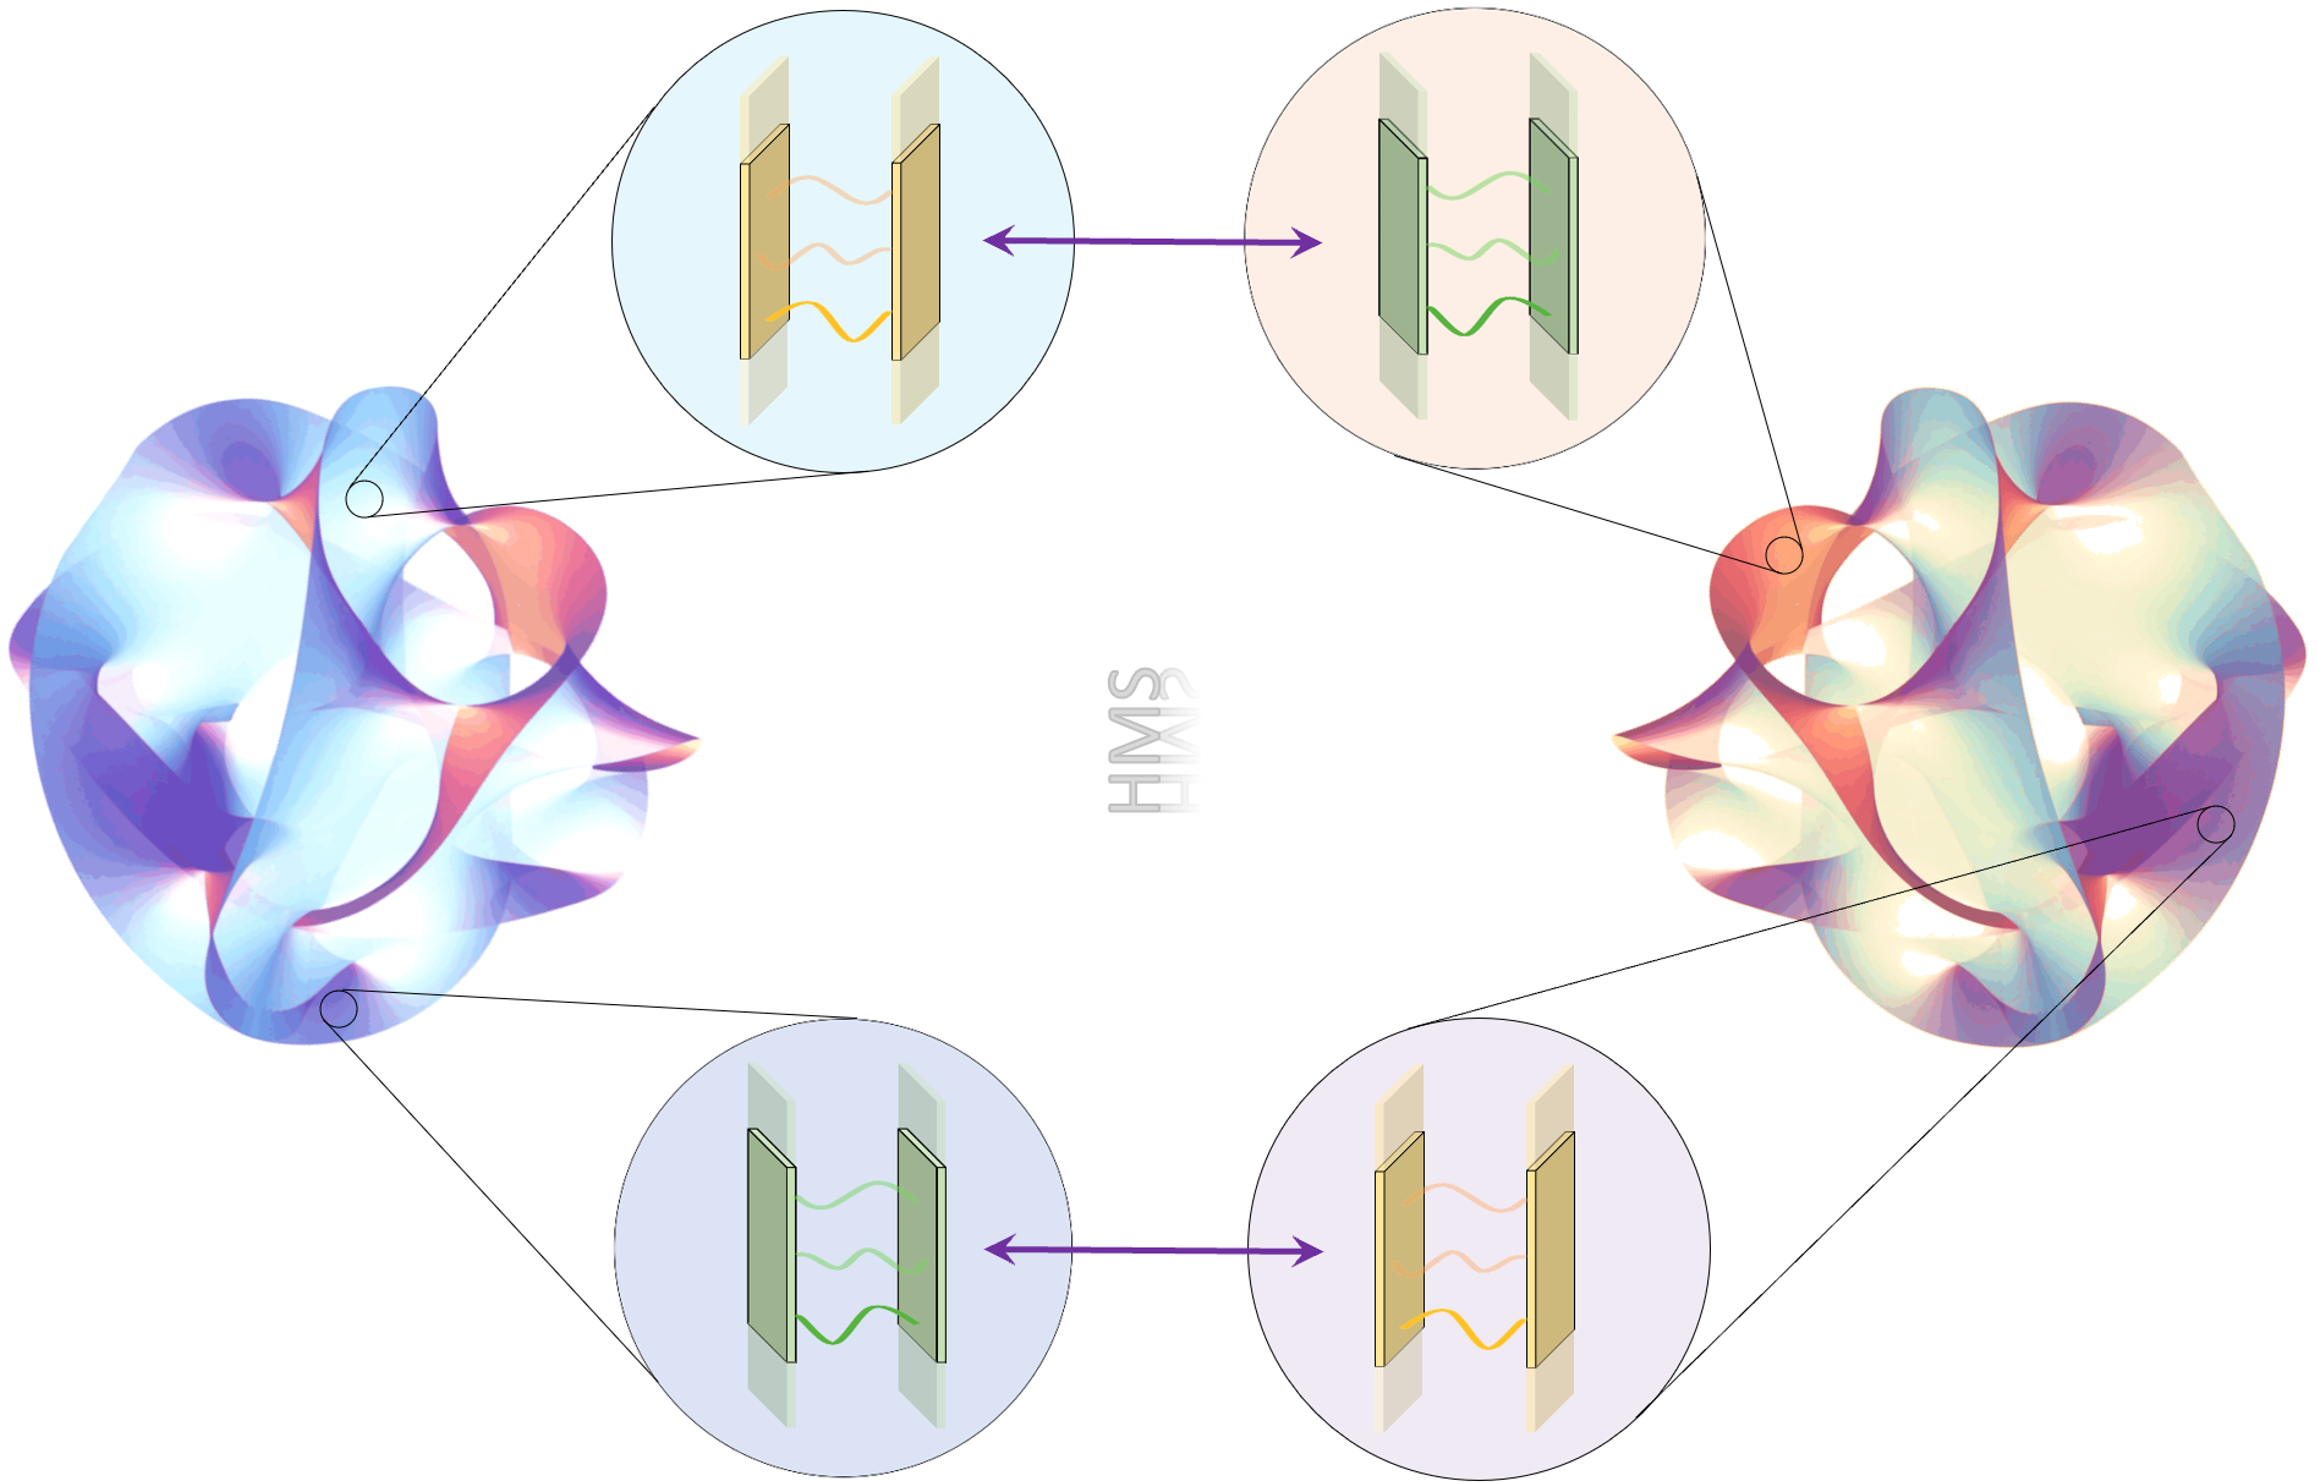
\includegraphics[width=1\textwidth]{HMScartoon.png}
\caption{一幅自解释的同调镜像对称猜想的卡通画。[来源：\begin{footnotesize}\texttt{https://plus.maths.org/content/hidden-dimensions}\end{footnotesize}]（原图位置：原 PDF 第 137 页）}
\end{figure}

\newpage
\thispagestyle{plain}
